\documentclass{beamer}



\usepackage{graphicx,subcaption,multicol}
\usepackage{float}
\usepackage{adjustbox}
\usepackage[table]{xcolor}
\usepackage{cite}
\usepackage{amsmath,amssymb,amsfonts}
\usepackage{algorithmic}
\usepackage{graphicx}
\usepackage{textcomp}
\usepackage{xcolor}
\usepackage{pgfplots}
\usepackage{fancyhdr}
\usepackage{color}
\usepackage{listings}


\title{COSC 3P93 Project Step 4}
\author{
    Parker TenBroeck 7376726\\
    pt21zs@brocku.ca
}
\date{\today}
\institute{\includegraphics[width=0.6\textwidth]{brock.jpg}}
%\date{2025}

\begin{document}
	
\frame{\titlepage}


\begin{frame}
	\frametitle{Intro}
	Rendering Triangle Meshes is the process of taking pre-defined or generated meshes and transforming it into a displayable image with a variety of effects
	\\~\\
	\centering
	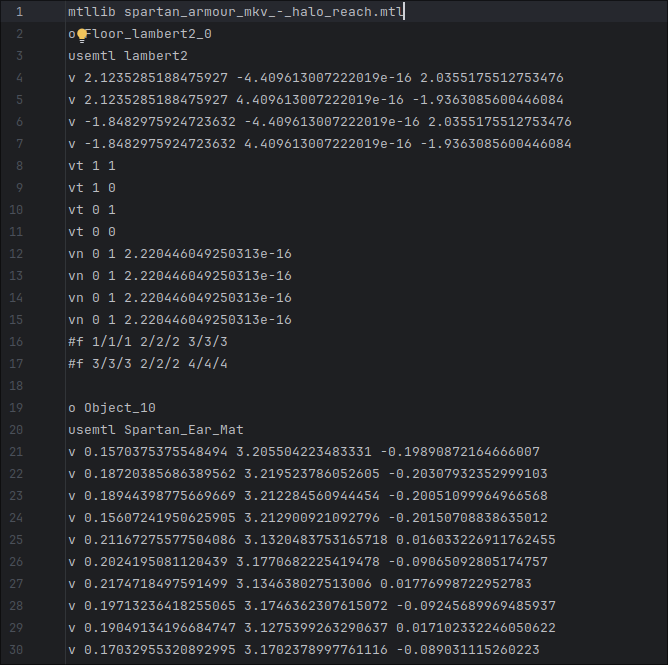
\includegraphics[width=0.23\linewidth]{halo_obj}
	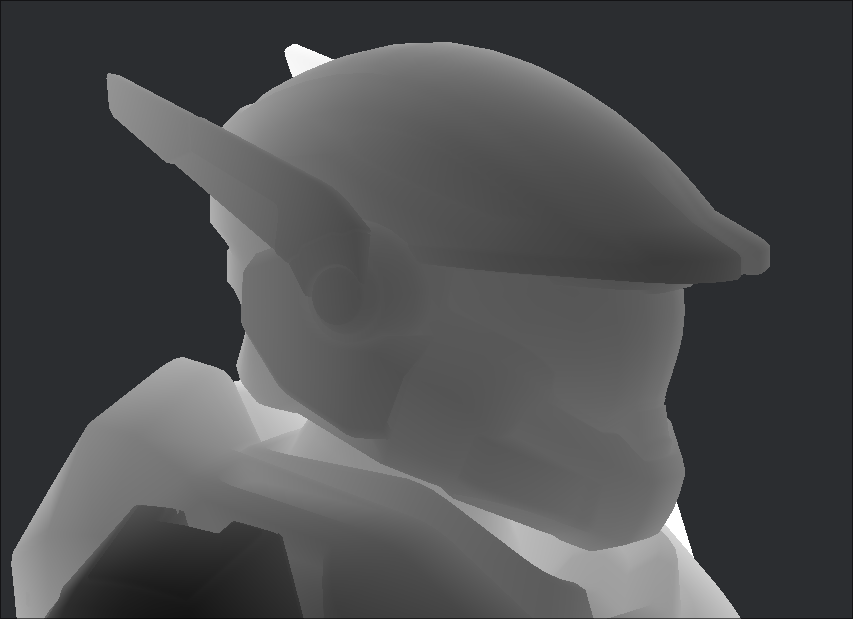
\includegraphics[width=0.23\linewidth]{halo_pre}
	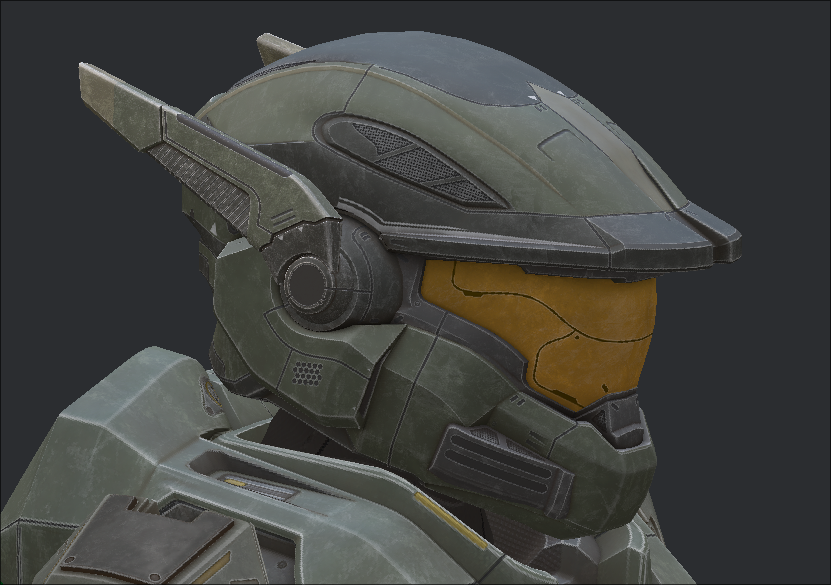
\includegraphics[width=0.23\linewidth]{halo_before}
	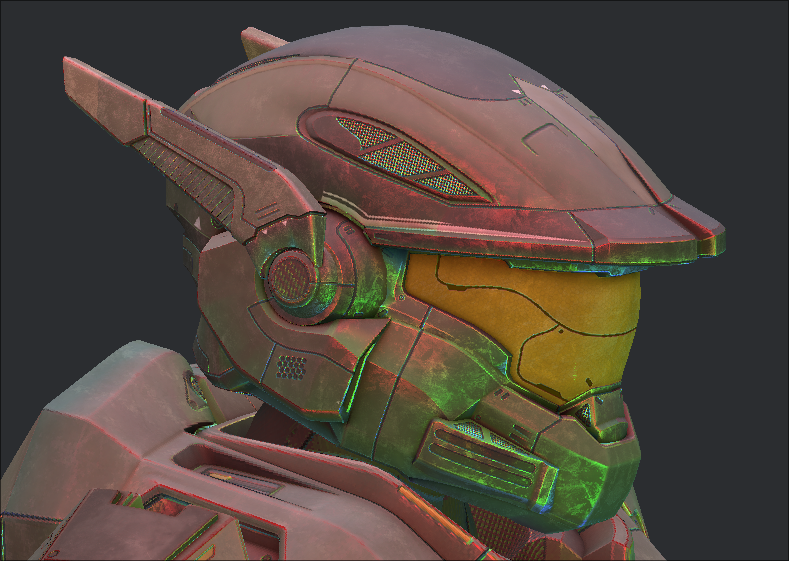
\includegraphics[width=0.23\linewidth]{halo_final}
	\\~\\
	You're probably familiar with this process if you've ever played a 3D game.
	
	
	
\end{frame}


\begin{frame}
	\frametitle{Problems}
	\textbf{Mesh Representation: } \\
	\hspace{1em} How do we represent a 3D mesh of triangles?
	\\
	\textbf{Projection: } \\
	\hspace{1em} How do we take 3D triangles and project them onto our screen?
	\\
	\textbf{Rasterization: } \\
	\hspace{1em} How do we draw these triangles to our screen taking into account the correct depths?
	\\
	\textbf{Lighting/Texturing: } \\
	\hspace{1em} how do we shade/texture our triangles efficiently?
	\\
	\textbf{Pixel Updates: }\\
	\hspace{1em} How do we ensure concurrent pixel writes select the closest pixel.
\end{frame}

\begin{frame}
	\frametitle{Solutions}
	\textbf{Mesh Representation: } \\
	\hspace{1em} Each mesh is a list of Faces, each face containing 3 3D points.
	\\
	\textbf{Projection: } \\
	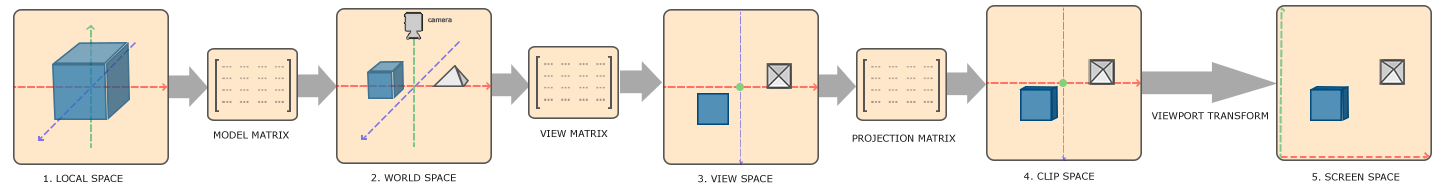
\includegraphics[width=1\linewidth]{coordinate_systems_long.png}
	\\
	\textbf{Rasterization: } \\
	\hspace{1em} Min/Max box over the trinalges projected screen space coordinates. Conversion to barycentric coordinate to calculate linearly interpolated pixel information. Using the projected Z value to determine depth of each pixel.
	\\
	\textbf{Lighting/Texturing: } \\
	\hspace{1em} Store needed information in pixel from material. Only calculate lighting on the pixels actually vidible(after all triangles have been rasterized). aka "Deferred rendering"
	\\
	\textbf{Pixel Updates: } \\
	\hspace{1em} Per Pixel Lock.
\end{frame}

\begin{frame}
	\frametitle{Tools and Libraries}
	STB libraries were used to read/write image files.\cite{stb-image}\cite{stb-image-write}\\~\\
	Tiny OBJ Loader was used to parse obj files for 3d models.\cite{tinyobjloader}\\~\\
	The 3D models used in the performance tests were sourced from SketchFab. \cite{bricks-model} \cite{halo-model}\\~\\
	Learn OpenGL was a incredible resource which all techniques in this project were based off. \cite{learn-open-gl}.
\end{frame}

\begin{frame}
	\frametitle{Responsibilities}
	Everything: Me, Myself, And I
\end{frame}

\begin{frame}
	\frametitle{Opportunities of Parallelism}
	
	\textbf{Per Frame: } \\
	\hspace{1em} Render seperate frames independently of eachother.
	\\~\\

	\textbf{Per Face(Triangle): } \\
	\hspace{1em} Projection and Rasterization.
	\\~\\
	
	\textbf{Per Fragment(Pixel): } \\
	\hspace{1em} Each Fragment in the image can have lighting and textures calculated independently of eachother.
\end{frame}

\begin{frame}
	\frametitle{Parallelism Degree}
	
	\textbf{MP: } \\
		\hspace{1em} Each fragment(pixel)'s lighting is calculated truly independently of eachother making this stage embarassingly parallel. Each triangle is projected independently of eachother but the rasterization step needs to ensure atomic stores for pixels in the frame buffer.\\~\\
	
	\textbf{MPI: } \\
	\hspace{1em} Embarrassingly parallel (for rendering). Each frame is rendered completely independently from eachother making each frame embarassingly parallel. 
\end{frame}

\begin{frame}
	\frametitle{Parallelism Design}
	
	\textbf{MP: } \\
	\begin{itemize}
		\item Triangle projection and rasterization is split statically per mesh. Through testing it was found that static scheduling works best in this case. 
		\item Fragment shader is split statically as all fragments require the same calculations.
	\end{itemize}
	
	
	\textbf{MPI: } Coordinator/Worker model.\\
	\begin{itemize}
		\item Coordinator: is responsible for initiating workers with input parameters (scene, resolution), providing model/image data if requested, and instructing workers which frames to render.
		\item Worker: Responsible for requesting needed model/texture data. Rendering requested frames.
	\end{itemize}
\end{frame}

\begin{frame}
	\frametitle{MP Implementation}
	
	Implementing MP was straight forward only requiring two parallel for clauses. The only synchronization needed was a spin-lock on each pixel to ensure updates happened synchronously\\~\\
	
	\centering
	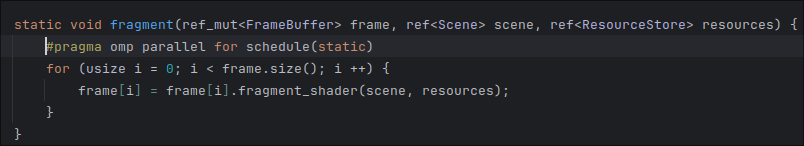
\includegraphics[width=0.7\linewidth]{fragment_par}
	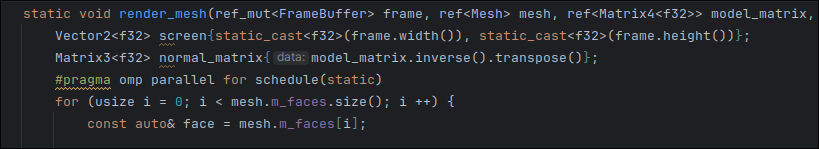
\includegraphics[width=0.7\linewidth]{vertex_par}
	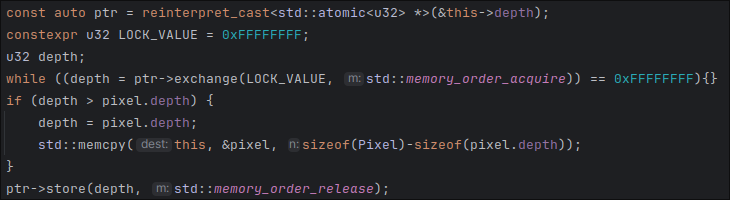
\includegraphics[width=0.7\linewidth]{spin_lock}
\end{frame}


\begin{frame}
	\frametitle{MPI Implementation}
	MPI was slightly more work necessitating workers to request files from the coordinator to load resources. Each worker notifies the coordinator when it is ready to start a new frame, and the coordinator responds with the frame number to render.
	\\~\\
	\centering
	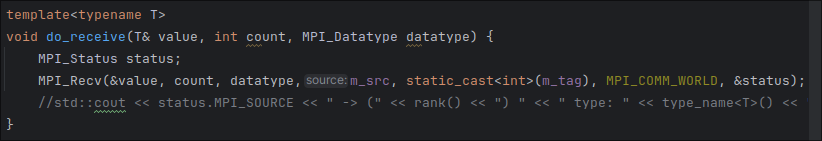
\includegraphics[width=0.7\linewidth]{mpi_recv}
	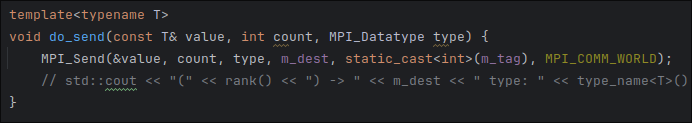
\includegraphics[width=0.7\linewidth]{mpi_send}	
\end{frame}


\begin{frame}
\frametitle{Performance Testing}


\begin{table}[H]
	\caption{Performance Bench Parameters}
	\centering
	\begin{tabular}{|c|c|}
		\hline
		Resolution& 360x240, 720x480, 1080x1920\\\hline
		Scenes/Triangles& Wavy(7212), Halo(42600), Bricks(752456)\\\hline
		Parallelism& Single Thread, MP/MPI(\#1, \#2, \#4, \#8, \#16)\\\hline
		Frames&300\\\hline
		CPU&AMD Ryzen 9 7950X (32) @ 5.883GHz\\\hline
		OS&NixOS 25.05 (Warbler) x86\_64\\\hline
		RAM&64GiB DDR5 \\\hline
		Compiler&clang version 19\\\hline
	\end{tabular}
	\label{table:performance-720-brick}
\end{table}
\end{frame}

\begin{frame}
	\begin{figure}[hbt!]
		\begin{subfigure}{.475\linewidth}
			\centering
			\textbf{\small Wavy}
			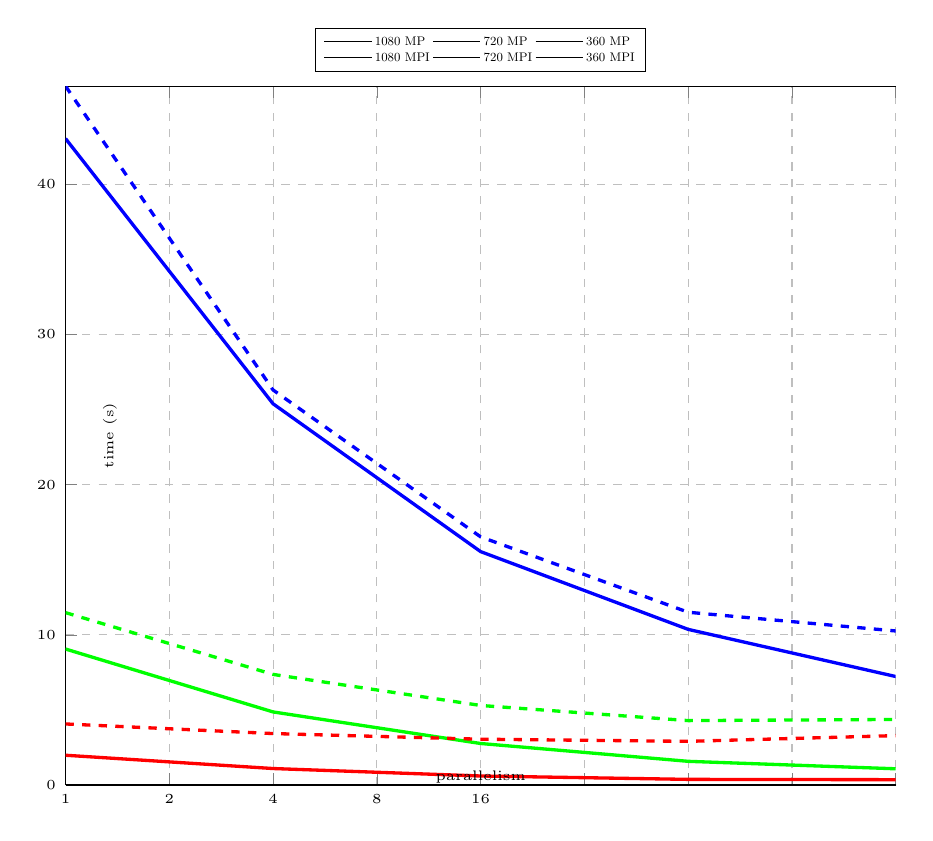
\begin{tikzpicture}[font=\tiny]
	\pgfplotsset{
		xmin=0, xmax=4,xticklabels={$0$,$1$,$2$,$4$,$8$,$16$},
		ytick distance=10, 
	}
	
	\begin{axis}[
		axis y line*=left,
		ymin=0.0, ymax=46.543007151,
		xlabel=parallelism,
		width=\textwidth,
		xlabel style={at={(ticklabel* cs:0.5,3)},anchor=south},
		ylabel=time (s),
		ylabel style={at={(ticklabel* cs:0.5,-10)},anchor=north},
		xmajorgrids=true,
		ymajorgrids=true,
		grid style=dashed,
		legend columns=3,
		legend style={nodes={scale=0.5}, at={(0.5,1.02)}, anchor=south},
		legend cell align={left}
		]
		
		\addlegendimage{/pgfplots/refstyle=mp1080}\addlegendentry{\small 1080 MP}
		\addlegendimage{/pgfplots/refstyle=mp720}\addlegendentry{\small 720 MP}
		\addlegendimage{/pgfplots/refstyle=mp360}\addlegendentry{\small 360 MP}
		
		\addlegendimage{/pgfplots/refstyle=mpi1080}\addlegendentry{\small 1080 MPI}
		\addlegendimage{/pgfplots/refstyle=mpi720}\addlegendentry{\small 720 MPI}
		\addlegendimage{/pgfplots/refstyle=mpi360}\addlegendentry{\small 360 MPI}
		
		\addplot[very thick,blue]
		coordinates{(0,43.048180543)(1,25.386438377)(2,15.542529991)(3,10.363813751)(4,7.224842113)}; \label{mp1080}
		
		\addplot[very thick,green]
		coordinates{(0,9.056300761)(1,4.867035691)(2,2.764863102)(3,1.577543137)(4,1.080982702)}; \label{mp720}
		
		\addplot[very thick,red]
		coordinates{(0,1.982921769)(1,1.097711781)(2,0.601079464)(3,0.375638776)(4,0.355170487)}; \label{mp360}
		
		\addplot[blue,dashed,very thick]
		coordinates{(0,46.543007151)(1,26.306487937)(2,16.525121953)(3,11.504767264)(4,10.25801139)}; \label{mpi1080}
		
		\addplot[green,dashed,very thick]
		coordinates{(0,11.479494068)(1,7.365175283)(2,5.29790582)(3,4.289567362)(4,4.365801786)};\label{mpi720}
		
		\addplot[red,dashed,very thick]
		coordinates{(0,4.066069377)(1,3.427016423)(2,3.050665738)(3,2.908242158)(4,3.289503899)    };\label{mpi360}
	\end{axis}
	
\end{tikzpicture}

			\label{plot:wavy}
		\end{subfigure}\hfill
		\begin{subfigure}{.475\linewidth}
			\centering
			\textbf{\small Halo}
			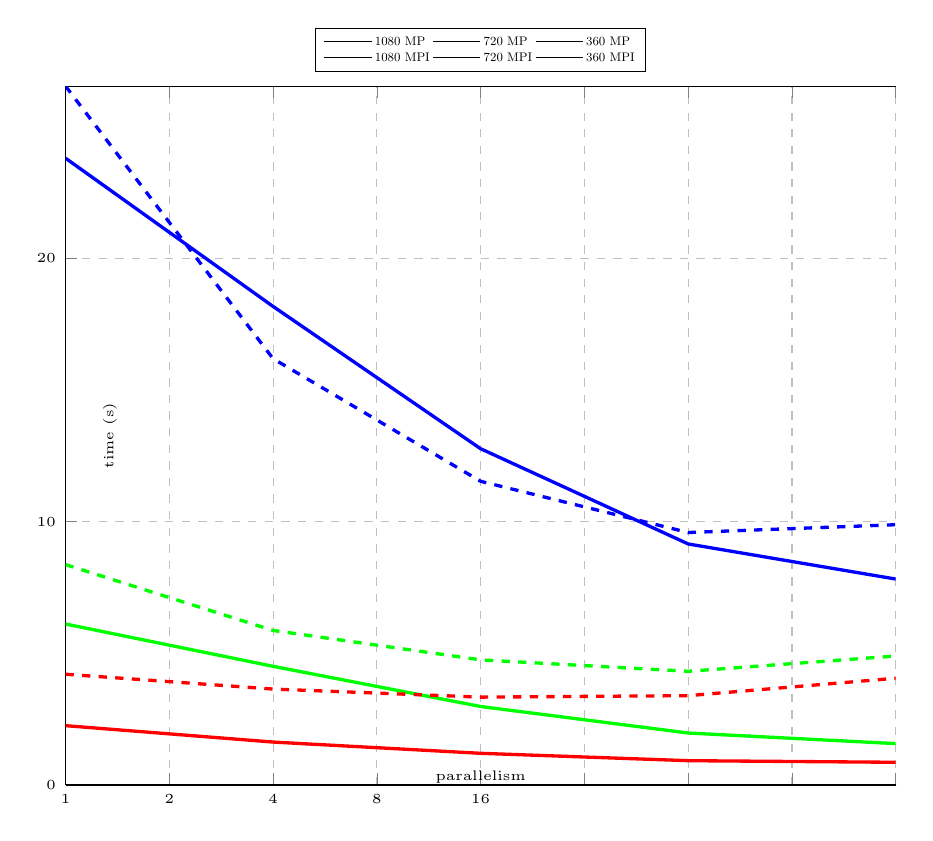
\begin{tikzpicture}[font=\tiny]
	\pgfplotsset{
		xmin=0, xmax=4,xticklabels={$0$,$1$,$2$,$4$,$8$,$16$},
		ytick distance=10, 
	}
	
	\begin{axis}[
		axis y line*=left,
		ymin=0.0, ymax=26.530752513,
		xlabel=parallelism,
		width=\textwidth,
		xlabel style={at={(ticklabel* cs:0.5,3)},anchor=south},
		ylabel=time (s),
		ylabel style={at={(ticklabel* cs:0.5,-10)},anchor=north},
		xmajorgrids=true,
		ymajorgrids=true,
		grid style=dashed,
   		legend columns=3, 
		legend style={nodes={scale=0.5}, at={(0.5,1.02)}, anchor=south},
		legend cell align={left}
		]
		
		\addlegendimage{/pgfplots/refstyle=mp1080}\addlegendentry{\small 1080 MP}
		\addlegendimage{/pgfplots/refstyle=mp720}\addlegendentry{\small 720 MP}
		\addlegendimage{/pgfplots/refstyle=mp360}\addlegendentry{\small 360 MP}
				\addlegendimage{/pgfplots/refstyle=mpi1080}\addlegendentry{\small 1080 MPI}
		\addlegendimage{/pgfplots/refstyle=mpi720}\addlegendentry{\small 720 MPI}
		\addlegendimage{/pgfplots/refstyle=mpi360}\addlegendentry{\small 360 MPI}
		
		\addplot[very thick,blue]
		coordinates{(0,23.793156579)(1,18.166806162)(2,12.765288078)(3,9.150427374)(4,7.818029104)}; \label{mp1080}
		
		\addplot[very thick,green]
		coordinates{(0,6.112349136)(1,4.505885243)(2,2.980769399)(3,1.974585661)(4,1.571729278)}; \label{mp720}
		
		\addplot[very thick,red]
		coordinates{(0,2.253051176)(1,1.631188636)(2,1.203912392)(3,0.923913927)(4,0.863365101)    }; \label{mp360}
		
				\addplot[blue,dashed,very thick]
		coordinates{(0,26.530752513)(1,16.183806498)(2,11.528919895)(3,9.584889808)(4,9.88103164)}; \label{mpi1080}
		
		\addplot[green,dashed,very thick]
		coordinates{(0,8.36632425)(1,5.867487997)(2,4.751012708)(3,4.317173429)(4,4.897371153)};\label{mpi720}
		
		\addplot[red,dashed,very thick]
		coordinates{(0,4.206369846)(1,3.642731525)(2,3.336637369)(3,3.391772581)(4,4.053479717)    };\label{mpi360}
	\end{axis}
	

	
\end{tikzpicture}
			\label{plot:halo}
		\end{subfigure}
		\medskip
		\begin{subfigure}{.475\linewidth}
			\centering
			\textbf{\small Bricks}
			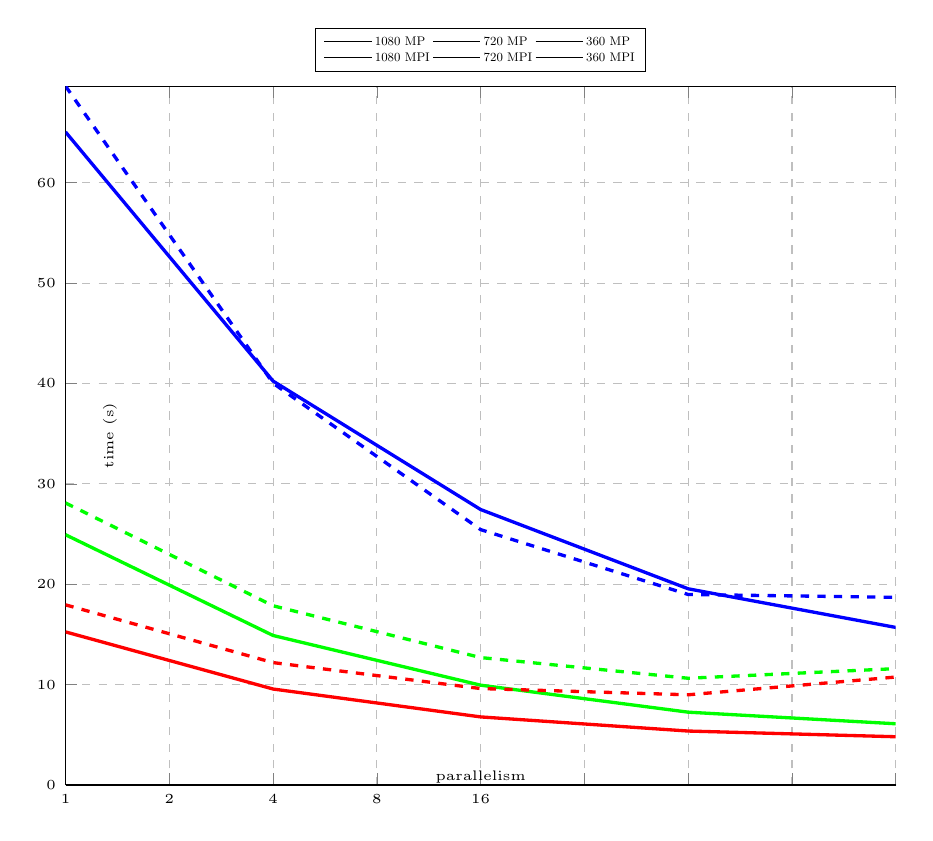
\begin{tikzpicture}[font=\tiny]
	\pgfplotsset{
		xmin=0, xmax=4,xticklabels={$0$,$1$,$2$,$4$,$8$,$16$},
		ytick distance=10, 
	}
	
	\begin{axis}[
		axis y line*=left,
		ymin=0.0, ymax=69.62863061,
		xlabel=parallelism,
		width=\textwidth,
		xlabel style={at={(ticklabel* cs:0.5,3)},anchor=south},
		ylabel=time (s),
		ylabel style={at={(ticklabel* cs:0.5,-10)},anchor=north},
		xmajorgrids=true,
		ymajorgrids=true,
		grid style=dashed,
		legend columns=3,
		legend style={nodes={scale=0.5}, at={(0.5,1.02)}, anchor=south},
		legend cell align={left}
		]
		
		\addlegendimage{/pgfplots/refstyle=mp1080}\addlegendentry{\small 1080 MP}
		\addlegendimage{/pgfplots/refstyle=mp720}\addlegendentry{\small 720 MP}
		\addlegendimage{/pgfplots/refstyle=mp360}\addlegendentry{\small 360 MP}
		
		\addlegendimage{/pgfplots/refstyle=mpi1080}\addlegendentry{\small 1080 MPI}
		\addlegendimage{/pgfplots/refstyle=mpi720}\addlegendentry{\small 720 MPI}
		\addlegendimage{/pgfplots/refstyle=mpi360}\addlegendentry{\small 360 MPI}
		
		\addplot[very thick,blue]
		coordinates{(0,65.057499734)(1,40.241821731)(2,27.44488066)(3,19.547062068)(4,15.699017481)}; \label{mp1080}
		
		\addplot[very thick,green]
		coordinates{(0,24.934087996)(1,14.896591606)(2,9.946441834)(3,7.256950884)(4,6.102009238)}; \label{mp720}
		
		\addplot[very thick,red]
		coordinates{(0,15.254607243)(1,9.563538488)(2,6.785384315)(3,5.377433791)(4,4.809364563)}; \label{mp360}
		
		\addplot[blue,dashed,very thick]
		coordinates{(0,69.62863061)(1,40.027101631)(2,25.441900785)(3,18.980813005)(4,18.697983013)}; \label{mpi1080}
		
		\addplot[green,dashed,very thick]
		coordinates{(0,28.101814261)(1,17.856819153)(2,12.697516728)(3,10.636469013)(4,11.59342073)};\label{mpi720}
		
		\addplot[red,dashed,very thick]
		coordinates{(0,17.949059101)(1,12.194260914)(2,9.610298317)(3,8.98890085)(4,10.75630727)    };\label{mpi360}
	\end{axis}
	
\end{tikzpicture}

			\label{plot:bricks}
		\end{subfigure}
	\end{figure}
\end{frame}

\newcommand{\SE}[2]{\footnotesize \(\begin{aligned}S&=#1\times \\[-5pt] E&=#2\% \end{aligned}\)}


\begin{frame}
	\frametitle{MP Performance Analysis}
	\centering
	\renewcommand{\arraystretch}{1.3}%
	\begin{tabular}{l|c c c c}
	&2&4&8&16\\
	\hline
	Bricks 360&\SE{1.60}{79.75}&\SE{2.25}{56.20}&\SE{2.84}{35.46}&\SE{3.17}{19.82}\\
	Bricks 720&\SE{1.67}{83.69}&\SE{2.51}{62.67}&\SE{3.44}{42.95}&\SE{4.09}{25.54}\\
	Bricks 1080&\SE{1.62}{80.83}&\SE{2.37}{59.26}&\SE{3.33}{41.60}&\SE{4.14}{25.90}\\
	Halo 360&\SE{1.38}{69.06}&\SE{1.87}{46.79}&\SE{2.44}{30.48}&\SE{2.61}{16.31}\\
	Halo 720&\SE{1.36}{67.83}&\SE{2.05}{51.26}&\SE{3.10}{38.69}&\SE{3.89}{24.31}\\
	Halo 1080&\SE{1.31}{65.49}&\SE{1.86}{46.60}&\SE{2.60}{32.50}&\SE{3.04}{19.02}\\
	Wavy 360&\SE{1.81}{90.32}&\SE{3.30}{82.47}&\SE{5.28}{65.98}&\SE{5.58}{34.89}\\
	Wavy 720&\SE{1.86}{93.04}&\SE{3.28}{81.89}&\SE{5.74}{71.76}&\SE{8.38}{52.36}\\
	Wavy 1080&\SE{1.70}{84.79}&\SE{2.77}{69.24}&\SE{4.15}{51.92}&\SE{5.96}{37.24}\\
	Average&\SE{1.59}{79.42}&\SE{2.47}{61.82}&\SE{3.66}{45.71}&\SE{4.54}{28.38}\\
\end{tabular}
\end{frame}

\begin{frame}
	\frametitle{MPI Performance Analysis}
	\centering
	\renewcommand{\arraystretch}{1.3}%
	\begin{tabular}{l|c c c c}
	&2&4&8&16\\
	\hline
	Bricks 360&\SE{1.47}{73.60}&\SE{1.87}{46.69}&\SE{2.00}{24.96}&\SE{1.67}{10.43}\\
	Bricks 720&\SE{1.57}{78.69}&\SE{2.21}{55.33}&\SE{2.64}{33.03}&\SE{2.42}{15.15}\\
	Bricks 1080&\SE{1.74}{86.98}&\SE{2.74}{68.42}&\SE{3.67}{45.85}&\SE{3.72}{23.27}\\
	Halo 360&\SE{1.15}{57.74}&\SE{1.26}{31.52}&\SE{1.24}{15.50}&\SE{1.04}{6.49}\\
	Halo 720&\SE{1.43}{71.29}&\SE{1.76}{44.02}&\SE{1.94}{24.22}&\SE{1.71}{10.68}\\
	Halo 1080&\SE{1.64}{81.97}&\SE{2.30}{57.53}&\SE{2.77}{34.60}&\SE{2.69}{16.78}\\
	Wavy 360&\SE{1.19}{59.32}&\SE{1.33}{33.32}&\SE{1.40}{17.48}&\SE{1.24}{7.73}\\
	Wavy 720&\SE{1.56}{77.93}&\SE{2.17}{54.17}&\SE{2.68}{33.45}&\SE{2.63}{16.43}\\
	Wavy 1080&\SE{1.77}{88.46}&\SE{2.82}{70.41}&\SE{4.05}{50.57}&\SE{4.54}{28.36}\\
	Average&\SE{1.50}{75.11}&\SE{2.05}{51.27}&\SE{2.49}{31.07}&\SE{2.41}{15.03}\\
\end{tabular}
\end{frame}



\begin{frame}
	\frametitle{Showcase}
	\href{https://www.cosc.brocku.ca/~pt21zs/demo.html}{https://www.cosc.brocku.ca/~pt21zs/demo.html}
\end{frame}

\begin{frame}
\frametitle{Citations}
\nocite{*}
\bibliographystyle{IEEEtran}
\bibliography{references}
\end{frame}

\end{document}
